\chapter{Conclusion}\label{chap:conclusion}
\dummy
\tikzsetnextfilename{n2vbowtie}
\begin{figure}[tbp]%
  \begin{tikzpicture}[node distance = .9ex, auto, remember picture]
    \tikzstyle{n2vcontainer} = [rectangle, draw, inner sep=.5ex, fill=clshade]
    \tikzstyle{n2vc} = [thick, circle, draw, fill=clnode, text width=1.5ex, text centered, minimum height=1.5ex, inner sep=0pt]
    
    % LEFT SIDE (INPUT LAYER)
    \node [n2vc, label=left:{$x_1$}] (c1) {};
    \node [n2vc, below=of c1, label=left:{$x_2$}] (c2) {};
    \node [n2vc, below=of c2, label=left:{$x_3$}] (c3) {};
    \node [n2vc, below=of c3, draw=none, fill=none] (c3-h) {};
    \node [n2vc, below=of c3-h, label=left:{$x_k$}] (c4) {};
    \node at ($(c3)!.5!(c4)$) {$\vphantom{\int^0}\smash[t]{\vdots}$};
    \node [n2vc, below=of c4, draw=none, fill=none] (c4-h) {};
    \node [n2vc, below=of c4-h, draw=none, fill=none] (c4-hh) {};
    \node [n2vc, below=of c4-hh, label=left:{$x_V$}] (c5) {};
    \node at ($(c4)!.5!(c5)$) {$\vphantom{\int^0}\smash[t]{\vdots}$};
    % Gray background box:
    \begin{scope}[on background layer]
      \node [n2vcontainer, fit=(c1)(c5)] (inputcontainer) {};
      \node[above] at (inputcontainer.north) {Input layer};
    \end{scope}
    
    % RIGHT SIDE (OUTPUT LAYER)
    \node [n2vc, right=7cm of c1,label=right:{$y_1$}] (o1) {};
    \node [n2vc, below=of o1, label=right:{$y_2$}] (o2) {};
    \node [n2vc, below=of o2, label=right:{$y_3$}] (o3) {};
    \node [n2vc, below=of o3, draw=none, fill=none] (o3-h) {};
    \node [n2vc, below=of o3-h, label=right:{$y_k$}] (o4) {};
    \node at ($(o3)!.5!(o4)$) {$\vphantom{\int^0}\smash[t]{\vdots}$};
    \node [n2vc, below=of o4, draw=none, fill=none] (o4-h) {};
    \node [n2vc, below=of o4-h, draw=none, fill=none] (o4-hh) {};
    \node [n2vc, below=of o4-hh, label=right:{$y_V$}] (o5) {};
    \node at ($(o4)!.5!(o5)$) {$\vphantom{\int^0}\smash[t]{\vdots}$};
    % Gray background box:
    \begin{scope}[on background layer]
      \node [n2vcontainer, fit=(o1)(o5)] (outputcontainer) {};
      \node[above] at (outputcontainer.north) {Output layer};
    \end{scope}
    
    % MIDDLE (HIDDEN LAYER)
    \begin{scope}[xshift=3.5cm, node distance = .7ex]
    %\node [draw] at ($(inputcontainer)!.5!(outputcontainer)$) {
    %  \begin{tikzpicture}[remember picture]
            \node [n2vc, yshift=-1.5em, label=right:{$h_1$}] (h1) {};
            \node [n2vc, below=of h1, label=right:{$h_2$}] (h2) {};
            \node [n2vc, below=of h2, draw=none, fill=none] (h3-h) {};
            \node [n2vc, below=of h3-h, label=right:{$h_i$}] (h4) {};
            \node at ($(h2)!.5!(h4)$) {$\vphantom{\int^0}\smash[t]{\vdots}$};
            \node [n2vc, below=of h4, draw=none, fill=none] (h4-h) {};
            \node [n2vc, below=of h4-h, label=right:{$h_N$}] (h5) {};
            \node at ($(h4)!.5!(h5)$) {$\vphantom{\int^0}\smash[t]{\vdots}$};
            % Gray background box:
            \begin{scope}[on background layer]
              \node [n2vcontainer, fit=(h1)(h5)] (hiddencontainer) {};
              \node[above, yshift=1.5em] at (hiddencontainer.north) {Hidden layer};
            \end{scope}
    %    \end{tikzpicture}
    %};
    \end{scope}
    
    % LINES MAKING THE BOW TIE
    \draw (inputcontainer.north east) -- (hiddencontainer.north west);
    \draw (inputcontainer.south east) -- (hiddencontainer.south west);
    \draw (outputcontainer.north west) -- (hiddencontainer.north east);
    \draw (outputcontainer.south west) -- (hiddencontainer.south east);
    
    
  \end{tikzpicture}
  \tikzsetnextfilename{n2vbowtieoverlay}
  \begin{tikzpicture}[remember picture, overlay]
    %\draw (inputcontainer.north) -- (outputcontainer.north);
  \end{tikzpicture}
\caption[short desc]{Text}%
\label{fig:n2v-figure}%
\end{figure}

\tikzsetnextfilename{n2vbowtie2}
\begin{figure}[tbp]%
  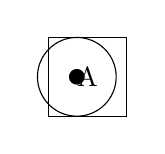
\begin{tikzpicture}[node distance = .9ex, auto]
        \tikzstyle{n2vc} = [thick, circle, draw, fill=clnode, text width=1.5ex, text centered, minimum height=1.5ex, inner sep=0pt]
          \node[matrix] (A) {
        \draw (0,0) rectangle (1,1); 
        \node at (0.5,0.5) {A}; \\
    };
    \node[matrix,left of=A] (B) 
    {
        \draw (0.5,0.5) circle (0.5);
        \fill (0.5,0.5) circle (0.1); \\
    };
    
  \end{tikzpicture}
\caption[short desc]{Text}%
\label{fig:n2v-figure}%
\end{figure}
